\documentclass[12pt,one side]{article}\usepackage[utf8]{inputenc}\usepackage[a4 paper]{geometry}\usepackage{graphicx, setspace, appendix, mathrsfs, enumerate,amsmath, amsfonts, array, tabularx, longtable, rotating, caption, mathtools}\usepackage[english]{babel}\renewcommand{\baselinestretch}{1.25}\doublespacing\title{Problem set 4}\author{Yao Luo}\begin{document}\maketitle
\begin{enumerate}
	\item The point estimates are presented in the following table:

	\begin{tabular}{c|c|c|c}
	\hline
	 & $MC_H(p)$ & $MC_L(p)$ & $MC_S(p)$\\
	\hline
	intercept & -120.92 & -94.04& 3.01\\
	slope& 1.06& 1.02&0.98\\
	\hline
	\end{tabular}

	Use the delta method to calculate standard errors:\\
	\[Var(\mu_H) = Var(\gamma_H) + Var(\delta_H)(\frac{\alpha}{\beta})^2 + (\frac{\delta_H}{\beta})^2Var(\alpha) + (\frac{\alpha\delta_H}{\beta^2})^2Var(\beta)\]
	\[SE(\mu_H) = \sqrt{Var(\mu_H)} \approx 22.440\]
	\[Var(\nu_H) = 4Var(\delta_H)\]
	\[SE(\nu_H) = \sqrt{Var(\nu_H)} \approx 0.037\]
	\item Plotting $D(p)$, $AIC_H(p)$, $MC_H(p)$ and data points in the same figure:
	\begin{figure}[h]
	\centering
	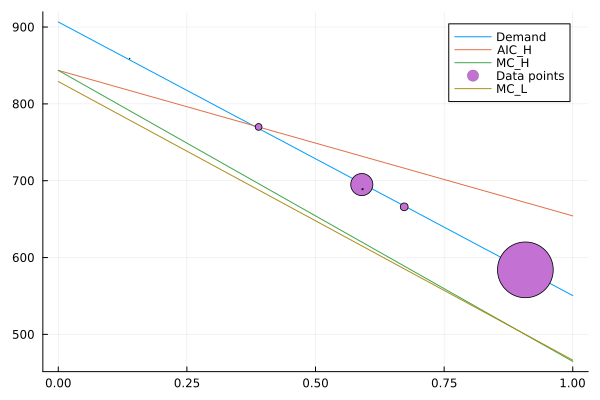
\includegraphics[width = 0.7\textwidth]{plot2.png}
	\end{figure}
	Since the marginal cost curve is downward sloping, this figure features adverse selection, where customers with the highest willingness to pay also have the highest expected costs.\\
	Efficient point: Demand curve intersects with the MC curve. \\
	Competitive equilibrium point: Demand curve intersects with $AIC_H$ curve, which we denote as point A.\\
	In the competitive market there would be underprovision of the high coverage plan because of adverse selection.\\
	DWL: The area to the right of vertical line going through point A and between the demand and $MC_H$ lines.
	\item The $MC_H$ curve lies above the $MC_L$ curve, but they are very close. If we fail to reject the null hypothesis of $MC_H \not= MC_L$, it implies there is moral hazard. If we reject the null hypothesis, we couldn't conclude that there is no moral hazard. We need to directly compare $MC_H$ and $MC_S$.
	\item Leave out $MC_L(p)$ and plot $MC_S(p)$. 
	\begin{figure}[h]
	\centering
	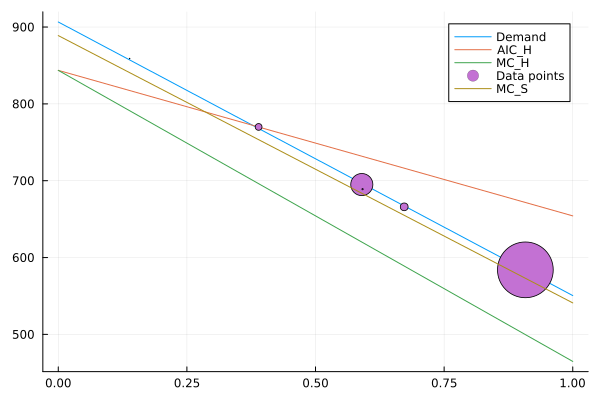
\includegraphics[width = 0.7\textwidth]{plot3.png}
	\end{figure}
	The $MC_S$ curve is above the $MC_H$ curve and they are quite far away depending on the point estimates. If we fail to reject that $MC_H \not= MC_S$, there exists moral hazard. If we reject it, it implies there is no moral hazard.
\end{enumerate}

\end{document}